\chapter{Introduction}
Welcome to your remote lab for ECE 380, Introduction to Feedback Control.
The in-lab portion of this course was designed to give you a hands-on
feel for control using analog circuits. Given the current climate, this is
clearly not possible in the way previously envisioned.

We persist. This lab is designed to run in MATLAB and Simulink. You will engage
in understanding, developing, executing and analyzing Simulink
diagrams that model and simulate control systems. Every lab, though
somewhat artificial, is
provided with brief motivation on how one can see this applied in a real
world problem. I hope I can help connect the abstract block diagrams of
Simulink with the real world for you.

Control systems is a very broad topic with a long history that even predates
the ideas discussed in this course. This course and lab covers the very basic
notion of control, the idea of the negative feedback loop, buttressed by
the mathematical tools of linear dynamical systems.

\section{MATLAB and Simulink}
MATLAB is a desktop numerical and symbolic
mathematics computing environment. We will not rely heavily on MATLAB
scripting itself and instead use Simulink but you should be familiar with
both environments. Please ensure that, when you are installing MATLAB, you
install
%
\begin{enumerate}[label=(\arabic*)]
  \item{
    MATLAB,
  }
  \item{
    Simulink,
  }
  \item{
    the Control Systems Toolbox,
  }
  \item{
    the Simulink Control Design,
  }
  \item{
    the DSP System Toolbox,
  }
  \item{
    the Signal Processing Toolbox,
  }
  \item{
    the Statistics and Machine Learning Toolbox and
  }
  \item{
    the Symbolic Math Toolbox.
  }
\end{enumerate}
%
Simulink is an add-on to MATLAB that allows you to design and simulate
systems (physical or otherwise) using block diagrams like in
Figure~\ref{fig:intro:1}.
%
\begin{figure}
  \centering
  \begin{tikzpicture}[x=1in, y=1in]
    \node [draw, block] (Controller) {\(K_p + K_i\frac{1}{s}\)};
    \node [draw, block, right=0.5 of Controller] (Plant) {\(\frac{1}{s}\)};
    \node [draw, summer, left=0.5 of Controller] (Sum) {};
    \node [below=0.5 of Sum] (BelowSum) {};

    \draw [arrow, signal]
      (Controller.east) -- (Plant.west);
    \draw [arrow, signal]
      (Plant.east)
      --
      +(0.35, 0)
      |-
      (BelowSum.base)
      --
      (Sum.south)
      node [below right, annotate] {\(-\)};
    \draw [arrow, signal]
      (Sum.east) -- (Controller.west);
    \draw [arrow, signal]
      ($(Sum.west)+1*(-0.5, 0)$) -- (Sum.west);
    \draw [arrow, signal]
      (Plant.east) -- +(0.7, 0);
  \end{tikzpicture}
  \caption[Example Feedback Diagram]{
    Example feedback diagram. The blocks are differential equations, expressed
    as a Laplace transfer function, that take an input signal and produce an
    output signal.
  }
  \label{fig:intro:1}
\end{figure}
%
Figure~\ref{fig:intro:1} can be replicated perfectly in Simulink.
That fact makes it easy for engineers to quickly design and verify
control designs. Simulink even supports direct interaction with
hardware but we will not utilize this feature.

The core of Simulink is the notion of a \emph{block}, maps that take an input
signal and produce an output signal.
The blocks we'll be concerned with primarily are \emph{gains}
(multiplier) depicted in Simulink like
\begin{center}
  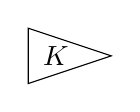
\begin{tikzpicture}[x=1em, y=1em]

    \draw
      (0, 0)
      --
      (3, 1)
      --
      (0, 2)
      --
      (0, 0)
      --
      (3, 1)
      node [at={(1, 1)}] {\(K\)};

  \end{tikzpicture}
\end{center}
and \emph{transfer functions} depicted in Simulink like
\begin{center}
  \begin{tikzpicture}[x=1em, y=1em]

    \node [draw, block] (Plant) {\(\frac{s+1}{s+2}\)};

  \end{tikzpicture}.
\end{center}
You may be provided template blocks to help you setup the Lab plant, the
system we wish to control; it will then be your task to analyze this block,
design a controller, and implement it by linking up blocks
in the appropriate feedback architecture.

% \section{Git Version Control}
% We will be using the \texttt{git} version control system in tandem with
% the Gitlab hosted on \url{git.uwaterloo.ca} to facilitate delivery of lab
% content and to give you a mechanism for
% \begin{enumerate}[label=(\arabic*)]
%   \item{tracking your temporary work, and}
%   \item{submitting your final work.}
% \end{enumerate}
% There is no requirement that you use git ``properly.'' If you are not
% comfortable using the terminal to perform git operations, you can use graphical
% tools like \href{https://www.sourcetreeapp.com/}{Sourcetree} or
% \href{https://www.gitkraken.com/git-client}{GitKraken}. You can even manually
% upload the files using the graphical web interface at \url{git.uwaterloo.ca}.
% As long as your able to download files from your repository and upload your
% solutions, I am happy. Having said that, it is an important skill in this
% day and age to understand how to use version control. This is a
% great opportunity to learn git!

\section{Lab Logistics and Deliverables}\label{intro:logistics}
Lab deadlines can be found in Table~\ref{tab:labcalendar}. Read carefully.
I have provided all times in both EDT as well as UTC.
Every lab requires you to complete a number of procedures described in
green boxes like
\begin{procedure}[]
  Here are some steps:
  \begin{enumerate}[label=(\arabic*)]
    \item{Yes here is step 1,}
    \item{oh wow step 2,}
    \item{really you are still reading this,}
    \item{you must be really bored,}
    \item{consider finding better things to do.}
  \end{enumerate}
\end{procedure}
\noindent
and deliverables described in red boxes like
\begin{deliverable}[]
  Here are some things you will need to save for your report.
\end{deliverable}
Procedures are simply steps you should follow that will eventually result in
a deliverable, which is something you must record and submit as part of your
report. Every lab chapter ends with a final summative deliverable, usually
consisting of a series of questions that you must answer.
%
All the deliverables should be packaged up in an organized way; ideally
they should be in your report in the order presented under headings directly
corresponding to the deliverable label (1.1, 1.2, etc.). If you want a sense
of how to format your report, please see a very basic LaTeX template that I
have created for you on Overleaf \href{https://www.overleaf.com/read/jnwwfmnvkgpx}{here}.
Your final report must be submitted as a PDF document on Learn.
Your grade is entirely based
on your report. Every lab has its own grading scheme, but the following
penalties apply equally to all labs:
\begin{itemize}
  \item{
    \(-5\%\) for not having a typeset document or for poor organization,
  }
  \item{
    \(-10\%\) for not submitting a PDF,
  }
  \item{
    \(-20\%\) within the first \texttt{24} hours it is late. After
    \texttt{24} hours, it becomes \(-100\%.\) If prior arrangements are made
    or a valid reason presented within a week from the missed deadline, this
    is waived. In no case will a lab report be accepted more than a week past
    the deadline; if a valid reason exists for being unable to hand in the lab
    within the week following the deadline, then the lab will be assigned a
    weight of zero and the remaining labs will be reweighted accordingly.
    \textbf{Contact the Lab Instructor for this.}
    All reports are due at \texttt{23:59:59 EDT} on the due date.
    All deadlines will be reported both
    in Eastern Daylight Time (\texttt{EDT}) and Coordinated Universal Time
    (\texttt{UTC})
    so that there can be no confusion on the deadline in case you are not
    in Waterloo.
  }
\end{itemize}
%
In terms of general style, I am a proponent of letter grade style
grading schemes for discussion questions.
Often grading is arbitrary and it can be hard to really pin down the value of
a question especially when the content has no obvious discrete points to
get correctly for the student and marker. I will have markers
rate these discussion answers on the scale shown in
Table~\ref{tab:letter-grading}.
%
\begin{table}
\centering
\begin{tabular}{r|c|l}
Value & Letter & Explanation\\ \hline
\(100\%\) & A+ & Meets Expectations.\\ \hline
\(90\%\)  & A & Meets Expectations. Answer could be Improved Upon. \\ \hline
\(80\%\) & B & Would Meet Expectations. Made Minor Mistakes.\\ \hline
\(60\%\) & C & Would Meet Expectations. Made a few Major Mistakes.\\ \hline
\(40\%\) & D & Fundamental Lack of Understanding in Attempt.\\ \hline
\(0\%\) & F & No Understanding or No Work Shown.
\end{tabular}
\caption[Letter Grading Scheme]{Letter grade with associated value and
description for how we assign the grade.}
\label{tab:letter-grading}
\end{table}
%
Minor mistakes are penalized quite steeply so check your work. Mistakes in
discussions usually amount to theoretical mistakes in understanding; empirical
mistakes are deducted in other rows and we will make an attempt to avoid double
(cascade) deductions. The letter grade \(A\) is reserved for when discussion
responses have no mistakes but a better explanation exists or an explanation
ought to be expanded upon. This is to prevent steep penalties for purely a
lack of insight.

%
\begin{table}
  \centering
  \begin{tabular}{c|c|c|l}
      & Release Date & Due Date & Grading Release Date\\ \hline
    Form Your
      &
      & \texttt{17 MAY 2359 EDT}
      & \\
    Group
      &
      & \texttt{18 MAY 0359 UTC}
      & \\ \hline
    Lab 1
      & \texttt{17 MAY 2359 EDT}
      & \texttt{24 MAY 2359 EDT}
      & {\color{blue}\texttt{31 MAY 2359 EDT}}\\
      & \texttt{18 MAY 0359 UTC}
      & \texttt{25 MAY 0359 UTC}
      & {\color{blue}\texttt{01 JUN 0359 UTC}}\\ \hline
    Lab 2
      & {\color{blue}\texttt{31 MAY 2359 EDT}}
      & {\color{blue}\texttt{07 JUN 2359 EDT}}
      & {\color{blue}\texttt{14 JUN 2359 EDT}}\\
      & {\color{blue}\texttt{01 JUN 0359 UTC}}
      & {\color{blue}\texttt{08 JUN 0359 UTC}}
      & {\color{blue}\texttt{15 JUN 0359 UTC}}\\ \hline
    Lab 3
      & {\color{blue}\texttt{14 JUN 2359 EDT}}
      & {\color{blue}\texttt{21 JUN 2359 EDT}}
      & {\color{blue}\texttt{28 JUN 2359 EDT}}\\
      & {\color{blue}\texttt{15 JUN 0359 UTC}}
      & {\color{blue}\texttt{22 JUN 0359 UTC}}
      & {\color{blue}\texttt{29 JUN 0359 UTC}}\\ \hline
    Lab 4
      & {\color{blue}\texttt{05 JUL 2359 EDT}}
      & {\color{blue}\texttt{12 JUL 2359 EDT}}
      & {\color{blue}\texttt{19 JUL 2359 EDT}}\\
      & {\color{blue}\texttt{06 JUL 0359 UTC}}
      & {\color{blue}\texttt{13 JUL 0359 UTC}}
      & {\color{blue}\texttt{20 JUL 0359 UTC}}\\ \hline
    Lab 5
      & {\color{blue}\texttt{26 JUL 2359 EDT}}
      & {\color{blue}\texttt{02 AUG 2359 EDT}}
      & {\color{blue}\texttt{09 AUG 2359 EDT}}\\
      & {\color{blue}\texttt{27 JUL 0359 UTC}}
      & {\color{blue}\texttt{03 AUG 0359 UTC}}
      & {\color{blue}\texttt{10 AUG 0359 UTC}}
  \end{tabular}
  \caption[Lab Calendar]{%
    Lab Calendar showing release dates, due dates and expected grading
    deadlines. Tentative dates are colored blue.
  }
  \label{tab:labcalendar}
\end{table}
